% ==============================
\section{lezione del 27-03-26}
\subsection{Polarizzazione del transitore BJT}\label{sub:polarizzazione_del_transitore_bjt} % (fold)
Nella scorsa lezione abbiamo visto il modello di \textbf{Ebers-Moll}, il quale 
ci impone di risolvere equazioni differenziale che talvolta possono risultare 
scomode o non pratiche. Vediamo adesso il comportamento del transitore bipolare 
e come si possono risolvere i cirucuiti applicando un modello semplificato. 

\begin{center}
    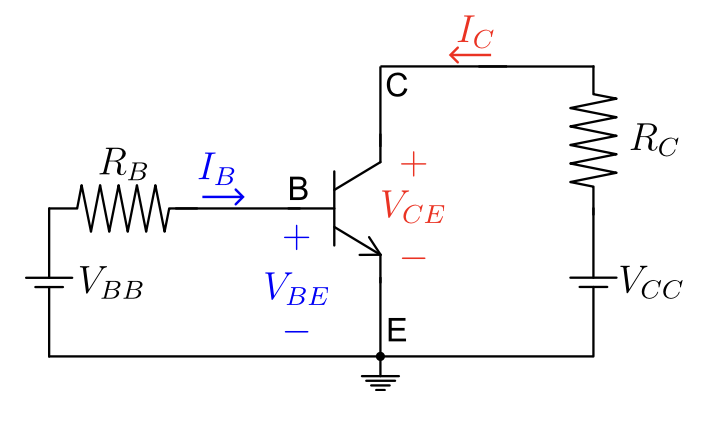
\includegraphics[scale=0.65]{../images/polarizzazione_transitore_bjt.png}
\end{center}

Analizziamo questo circuito cercando di determinare il punto di riposo ($V_{BE_Q}, I_{B_Q}, V_{CE_Q}, I_{C_Q}$) del transitore.
Abbiamo diversi approcci: 
\begin{itemize}
    \item \textbf{Analitici}: modello di Ebers-Moll o il modello semplificato
    \item \textbf{Grafici}: tracciatura della retta di carico sulle caratteristiche
\end{itemize}

Scriviamo adesso le equazioni alle due maglie del circuito
\[
    \begin{cases}
        V_{BB} = R_B I_B + V_{BE} \\ 
        V_{CC} = R_C I_C + V_{CE} \\ 
    \end{cases}
\]
e ricordiamo le \textit{equazioni caratteristiche} del BJT

\[
    \begin{cases}
        I_B = f(V_{BE}, V_{CE}) \\ 
        I_C = g(V_{CE}, I_B) \\ 
    \end{cases}
\]
\subsubsection{Modello grafico}\label{sec:modello_grafico} % (fold)

Utilizziamo ora il medoto gradico per trovare, senza commettere errori di approssimazione i 
valori del punto di riposo
\begin{center}
    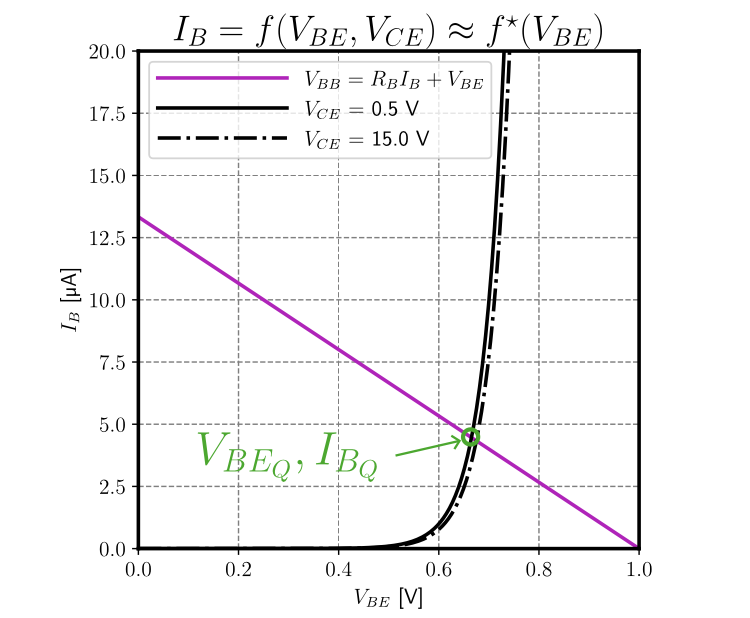
\includegraphics[scale=0.75]{../images/grafico_polarizzzazione_transitore_bjt_ingresso.png}
\end{center}
Notiamo dal grafico che \textit{l'effetto Early} è trascurabile sulle caratteristiche di ingresso
($V_{BE_Q}, I_{B_Q}$) che determinamo per via grafica. Sempre con lo stesso metodo otteniamo le caratteristiche 
in uscita ($_{C_Q}, V_{CE_Q}$)
\begin{center}
    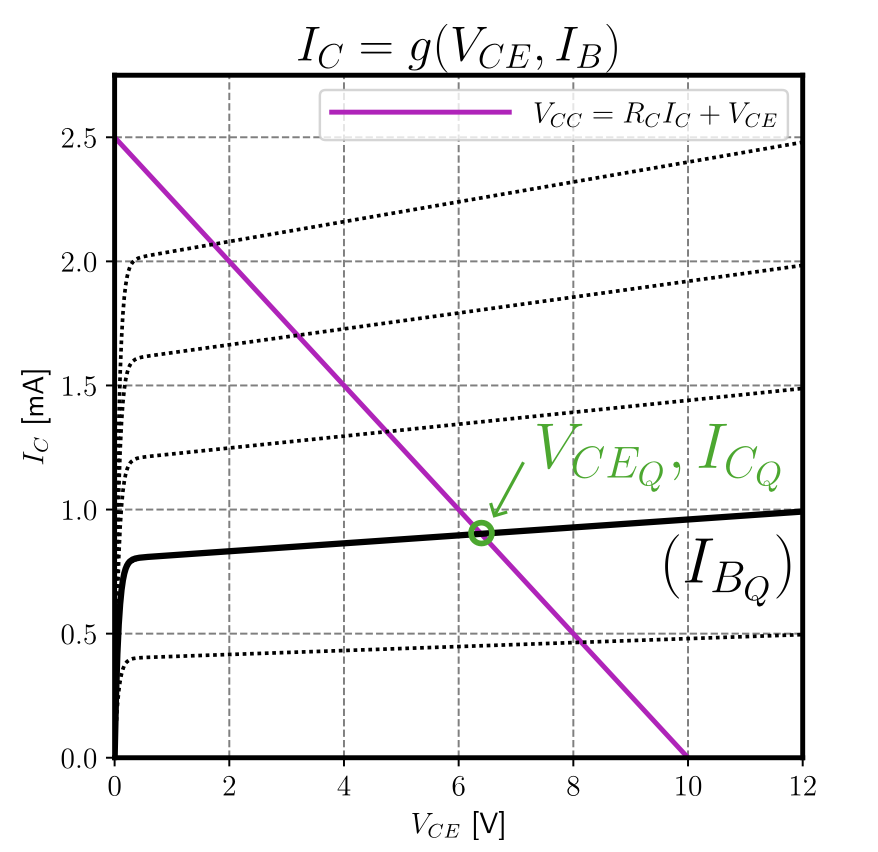
\includegraphics[scale=0.55]{../images/grafico_polarizzzazione_transitore_bjt_uscita.png}
\end{center}
% subsubsection Modello grafico (end)
\subsubsection{Modello analitico}\label{sec:modello_analitico} % (fold)
Partiamo adesso con la risoluzione del medesimo circutio con il \textit{medoto analitico}. 
Rimangono comunque le considerazioni fatte prima, ovvero che l'effetto Early è trascurabile quindi 
\[
    I_B = (1 - \alpha_F)I_{ES}e^{\frac{V_{BE_Q}}{V_T}}
\] 
Sotituendo quanto appena trovato nell'equazione della retta di carico otteniamo
\[
    V_{BB} = R_B(1 - \alpha_F)I_{ES}e^{\frac{V_{BE_Q}}{V_T}} + V_{BE_Q}
\]
Notiamo subito che questa è un equazione trascendentale con incognita $V_{BE}$, andiamo quindi
ad utlizzare il \textbf{modello analitico semplificato} portandoci in determinate condizioni 
\begin{itemize}
    \item  \textit{Modello a caduta costante della giunzione BE }(ZAD):
        \[
            V^*_{BE_Q} = V_{\gamma} \approx 0.7 V
        \]
        Sostituiamo addesso, come prima, quanto appena trovato nell'equazione della retta di carico
        \[
            I^*_{B_Q} = \frac{V_{BB}-V_{\gamma}}{R_B}
        \]
        Ovviamente questo medoto commette un errore di approssimazione ma ci da il vantaggio 
        di poter risolvere il circuto utilizzando solo carta e penna.
        Notiamo anche che l'effetto Early viene trascurato anche sulla caratteristica di uscita
        quindi si una la semplice relazione 
        \[
            I^*_{C_Q} = \beta_F I^*_{B_Q}
        \]
        sostituendo otteniamo la seguente relazione 
        \[
            V^*_{CE_Q} = V_{CC} - R_C\beta_FI^*_{B_Q}, \quad \text{verifico}: V^*_{VE_Q} > V_{CE,SAT} \approx 0.2 V
        \]
        Abbiamo quindi trovato il punto di riposo approssimato ($V^*_{BE_Q}, I^*_{B_Q}, V^*_{CE_Q}, I^*_{C_Q}$)
\end{itemize}
% subsubsection Modello analitico (end)
% subsection Polarizzazione del transitore BJT (end)
\subsection{Risoluzione di circuti con il transitore bipolare}\label{sub:risoluzione_di_circuti_con_il_transitore_bipolare} % (fold)
Come per il diodo non possiamo sapere a priori in quale fra i tre stati possibili si trova il transitore
prima di risolvere il circuito, dobbiamo quindi fare delle ipoesi, risolvere il circuito e poi verificare le ipotesi fatte. 
Questa tabella riassume i vari stati del transitore bipolare in entrabe le configurazione e quali sono le verifiche da fare. 
\begin{center}
    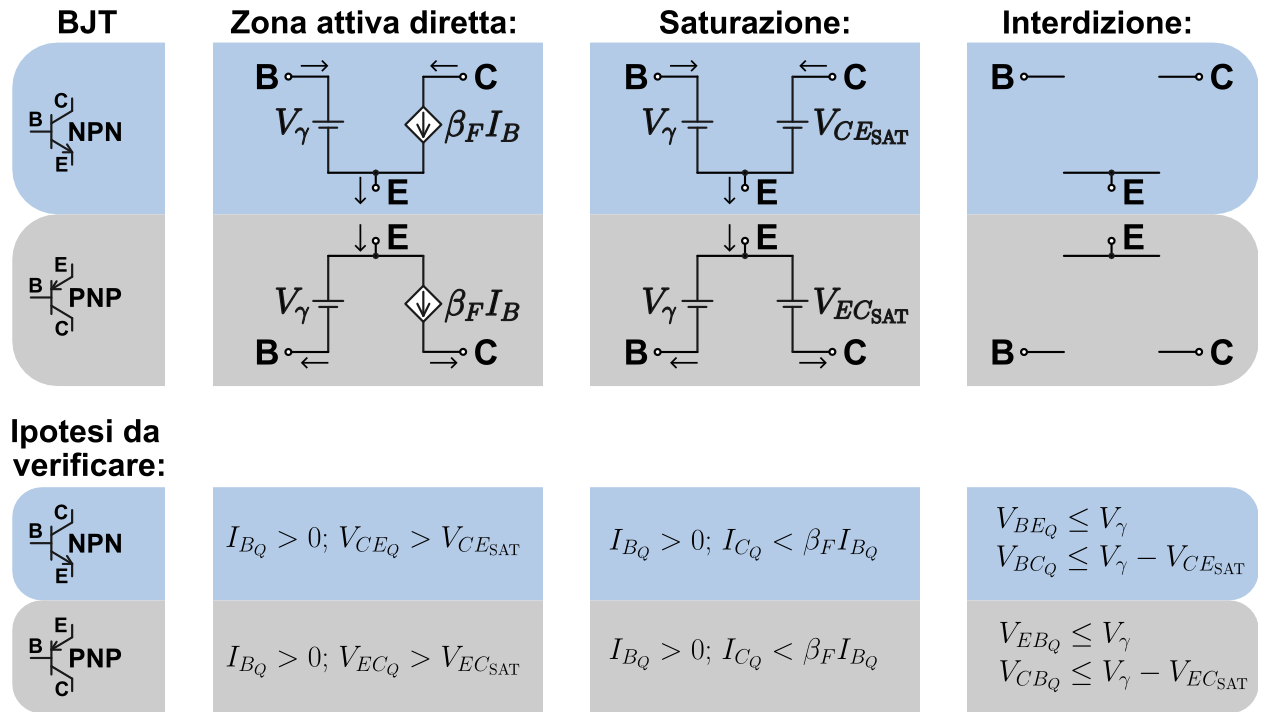
\includegraphics[scale=0.55]{../images/tabella_ipotesi_trasitore_bjt.png}
\end{center}
% subsection Risoluzione di circuti con il transitore bipolare (end)